\chapter{Definition and Literature Review}
\label{Chapter2}

% 转折
% \subsubsection{Approximate Bayesian Inference Intuition}
\section{Definition}

\section{Bayesian Inference Paradigm}
\label{bayeisanP}
\textbf{Why Bayesian}
Bayesian Inference approaches shares numerous advantages in statistic community and applicationa areas, particularly for the circumstance when there is lack of data. An appropriate prior choice can be beneficial in aforementioned case, especially for medical problem where the amount of effective data is extremely rare and untenable. Additionally, unlike frequentist inference approaches which treat parameter estimate as a fixed value, Bayesian Inference approaches regard parameter estimate as a random variable that have probability distribution, which means interval estimate and error variance would be generated for capturing uncertainty, offering  belief and confidence for interpretating parameter estimates.

\textbf{Bayesian Inference Intuition}
Bayesian inference approach stems from the Bayes rule, which is defined as Equation (\ref{eq:Bayesrule}) based on theory developed by \cite{Beech1959}. Suppose $\theta$ is our model parameter of interest, $\mathcal{D}$ is data, then $p(\theta)$ is known as prior distribution, which offers pre-existing knowledge or information about $\theta$. Posterior distribution $p(\theta|\mathcal{D})$ refers to the likelihood conditioning on the data $\mathcal{D}$.
Incorporating information from current data and prior knowledge, posterior distribution can be then inferred and simplified to Equation (\ref{eq:simBayesrule}) since $p(\mathcal{D})$ is equal to constant and is also insignificant to know overall posterior distribution.
\begin{equation}
	p(\theta|\mathcal{D}) \propto p(\mathcal{D}|\theta)p(\theta),
	\label{eq:simBayesrule}
\end{equation}




\section{Least Absolute Shrinkage and Selection Operator(LASSO) penalized regression}
\subsection{Lasso penalty formulation}
The constraint form of lasso can be shown by Equation \ref{eq:lasso2}, where $t \geq 0$ is denoted as a tuning term $t$, regression coefficient is $\beta$, $||\beta||_1$ is the $l_1$ norm of beta, $||\beta||_2$ is the $l_2$ norm of $\beta$, data matrix is $X$, response variable is $y$. The estimation for lasso estimate $\hat{\beta}_{lasso}$ is defined by Equation \ref{eq:lasso2}. 

\begin{equation}
	\label{eq:lasso2}
	\hat{\beta}_{lasso} = \underset{\beta}{\operatorname{argmin}} ||y-X\beta||_2, s.t. ||\beta||_1 \leq t, t \geq 0.
\end{equation}
In order to transform constraint form of lasso to penalty form, Lagranage multiplier method, as a pivotal technique from transforming a constraint optimization system into an unconstrained penalty formulation of system has been used. The Lagrangian function for constrained Lasso Regression is constructed by Equation \ref{eq:lagrangelasso}
\begin{equation}
	\label{eq:lagrangelasso}
	\mathcal{L}(\beta,\lambda) =  ||y-X\beta||_2 + \lambda||\beta||_1 - \lambda t, \lambda \geq 0
\end{equation}
 Since the objective function contains a quadratic term $||y-X\beta||_2$ with a linear term $\lambda||\beta||_1 - \lambda t)$, leading to a convex optimization problem. Due to strong duality theorem in convex optimization system, therefore the penalty formulation of lasso regression can be deduced as Equation \ref{eq:lasso1}, is equivalent to constraint form \ref{eq:lasso2} after ignoring the unaffected constant $-\lambda t$.


Graphical demonstration of the lasso for Equation \ref{eq:lasso2} and Equation \ref{eq:lasso1} can also be found on the left hand side of the Figure \ref{fig:lassodemo}, where the squared constraint set is drawn, in addition to the contour line of regression coefficient. Given that $\lambda$ is set as penalty term that control the strength of penalization, larger penalization facilitate a more sparse solution, so that further enclosing the estimated coefficient to lies on the axis of each parameter as shown in Figure \ref{fig:lassodemo}. Lasso regression coefficient would have higher chance to render the contour line of $\beta$ intersect with the corner of the squared constraint set, causing the occurrence of sparse estimated regression coefficient. Compared with the ridge regression where a sum of square of penalty term is yielded instead on the right side of Figure \ref{fig:lassodemo}, ridge regression tends to gain a non-sparse solution due to circled constraint set for $\beta$.

\begin{figure}
	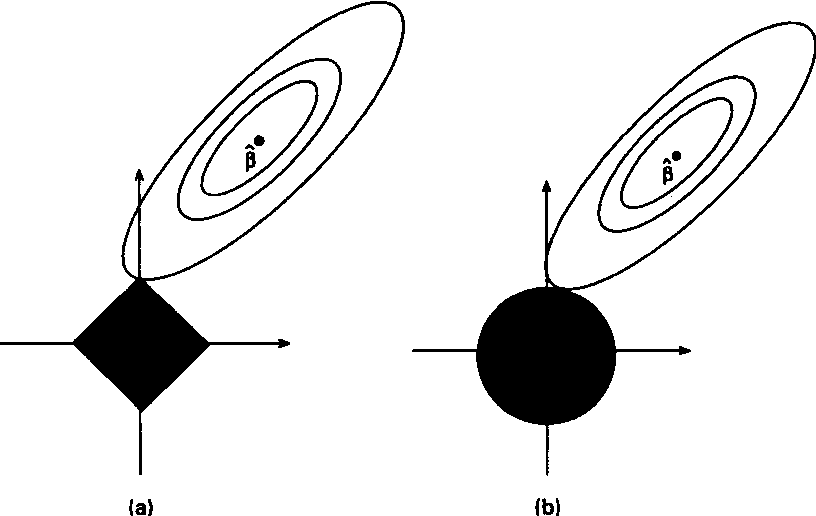
\includegraphics[width=\linewidth]{lassodemo}
	\caption{Graphical comparison between lasso regression and ridge regression}
	\label{fig:lassodemo}
\end{figure}

\textbf{Problem}
In addition, the optimal estimated $\beta_{lasso}$ can be generated by taking the derivative with respect to $\beta$ and solving the normal equation, denoted as Equation (\ref{eq:lassosolution}).
In addition, lasso estimated can be efficiently computed via Least Angle Regression algorithm by

\subsection{Bayesian Lasso regression}

Gbbs Sampler





% \section{Bayesian Paradigm}
\section{Expectation Maximization}
\subsection{Bayesian Expectation Maximization}

\section{Markov Chain Monte Carlo(MCMC)}
\label{MCMC}

\subsection{Metropolis–Hastings (MH) Algorithm}
\subsection{Gibbs Sampler}

\section{Variational Inference}
\label{VI}

\subsection{Mean Field Variational Bayes(MFVB)}
Suppose there are $n$ number of parameters, then MFVB assumes target distribution $q(\theta)$ is the product of single factorization of each parameter distribution $q_i(\theta_i)$, due to simplicity of product density form. 
\begin{equation}
	q(\theta) = \prod_{i=1}^{n} q_i(\theta_i)
\end{equation}
To measure the similarity between true distribution and target distribution, KL divergence metric is selected to produce

\begin{equation}
	KL(q(x)||p(x|\mathcal{D})) 
\end{equation}

\subsection{MFVB for Bayesian Lasso}






